Knowing model's uncertainty is crucial in safety-critical applications such as medical diagnosis, autonomous driving, etc. The output probability (softmax) of standard neural networks is typically not reliable. For example, deep neural nets can be overconfident for unrecognizable images. In these cases, the uncertainty should grow away from the typical data seen, but it doesn't.\\
For regression NNs, the uncertainty should look something like the following:
\begin{figure}[h!]
    \centering
    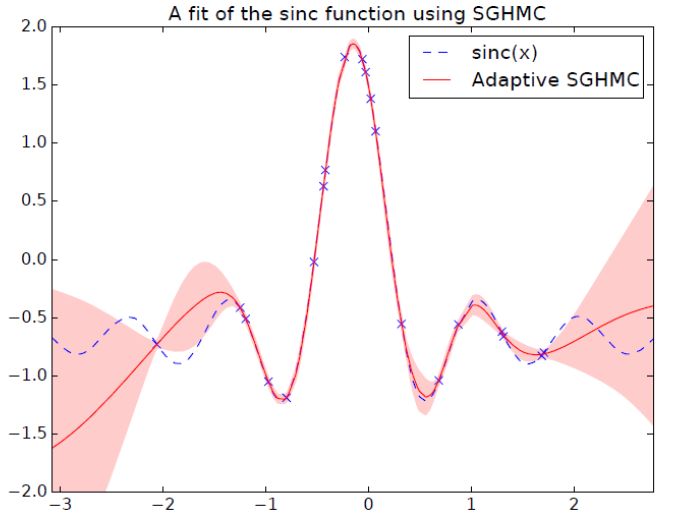
\includegraphics[width=0.5\textwidth]{uncertain.png}
\end{figure}

There are several types of uncertainty:
\begin{enumerate}
    \item \b{Aleatoric:} Intrinsic observation (data) noise.
    \item \b{Epistemic:} Uncertainty about the model, can be reduced by more data.
\end{enumerate}

\definition{Being Bayesian about NNs means dealing will all sources of parameter uncertainty: As more than one weight vector can explain the observed data, we need to take into account all possible explanations.}

\subsection{DNGO Model}
The DNGO model aims at being Bayesian at least about the output layer. DNGO first trains a neural network on a given dataset and use the feature vector obtained in the last hidden layer as basis functions of the Bayesian linear regression.

\subsection{Bayesian Neural Networks}
Given data \f{\mathcal{D}=(X,y)}, parameters \f{\theta}, a prior distribution \f{p(\theta)} and a likelihood \f{p(y|X, \theta)}, the core part of Bayesian Neural Networks is to compute the posterior distribution:
\cf{
    p(\theta|\mathcal{D}) = p(\theta|X,y) = \frac{p(y|X,\theta)p(\theta)}{p(y|X)} = \frac{p(y|X,\theta)p(\theta)}{\int p(y|X,\theta)p(\theta)d\theta}
}
\b{Problem:} Since the mean of \f{p(y|X,\theta)} is not a linear function of \f{\theta} and Gaussians are not closed under non-linear mappings, the posterior is not a Gaussian anymore. Approximating the posterior requires variational inference or the  Markov-Chain-Monte-Carlo method.

\subsection{Variational Inference}
Variational Inference (VI) is an optimization-based method for approximating intractable probability distributions in Bayesian inference. Instead of directly computing a complex posterior distribution \( p(z \mid x) \), VI approximates it with a simpler distribution \( q(z \mid \lambda) \) by minimizing the Kullback-Leibler (KL) divergence:
\[
q^*(z) = \arg\min_{q \in \mathcal{Q}} D_{\text{KL}}(q(z \mid \lambda) \parallel p(z \mid x)).
\]
This converts Bayesian inference into an optimization problem, making it computationally feasible for high-dimensional models.\\
In order to minimize this KL-Divergence w.r.t to \f{\theta}, we only need to maximize the ELBO. ELBO embodies a trade-off between satisfying the complexity of the data and satisfying the simplicity of the prior. ELBO is very popular since it approximates the true posterior with the variational posterior and therefore replaces the diffcult integral.

\subsection{Markov-Chain-Monte-Carlo (MCMC) Method}
Another posterior estimation is performed by MCMC. MCMC samples each weights according to a
proposal distribution or transition distribution \f{p(w_{t+1}|w_t)} and moves around the space while accepting or rejecting the proposal from the distribution. Since the next state is determined only by the current state, it is called Markov-chain. For the nal sampling, we use every \f{t}-th sample from the history to avoid the correlation between samples close to each other in terms of time steps. The goal of the sampling is to identify the stationary distribution \f{\pi} that is ideally the posterior distribution
\f{p(w|\mathcal{D})}. The sufficient condition for a stationary distribution to exist is that the detailed balance \f{\pi(w_t)p(w_{t+1}|w_t)=\pi(w_{t+1})p(w_t|w_{t+1})}. In practice, even when the detailed balance is satisfied, it may still take time to reach the stationary distribution. This time (from the beginning) is called mixing time. Intuitively, the distribution reaches the stationary distribution when the chain forgets the beginning states. Therefore, we take samples after a burning-in phase and the length of the burn-in phase is a hyperparameter.


\subsection{Prior-Fitted Networks (PFNs)}
PFNs are neural networks trained to approximate Bayesian inference by learning a prior distribution over possible data-generating processes. Instead of traditional training on a fixed dataset, PFNs are trained on a diverse set of synthetic tasks sampled from a prior, enabling them to generalize to new tasks without gradient-based fine-tuning. This allows PFNs to perform rapid adaptation in a Bayesian manner while leveraging neural network expressiveness.\\
PFNs might be a disruptive alternative to variational inference and MCMC.


\subsection{Output Ensembling}
Construct an ensemble of \f{M} neural networks on the training data. For each test data point \f{x} predict with each of the \f{M} networks and combine the outputs to obtain probabilistic predictions:
\cf{
    f(x) = \frac{1}{M}\sum_{i=1}^{M}f_i(x),\quad\text{(classification case)}
}
where \f{f_i(x)} is the output of the \f{i}-th network. For the regression case we can compute the empirical mean and variance across the predictions like so:
\cf{
    \mu_x = \frac{1}{M}\sum_{i=1}^{M}f_i(x)
}
\cf{
    \sigma_x^2 = \frac{1}{M}\sum_{i=1}^{M}(f_i(x)-\mu_x)^2
}

The \f{M}-Ensemble can be created in different ways: via dropout (simply by sampling \f{M} dropout masks), via MCMC, via different random seeds for SGD initialization, etc.

\subsection{The Estimation of Parametric Models}
We can train a network with weight \f{\theta} to output the parameters \f{w} of a parametric model \f{p(y|x,w)}. Most commonly we have the network output \f{\mu} and \f{\log(\sigma^2)} of a Gaussian \f{\mathcal{N}(\mu, \sigma^2)}.\\
This can be achieved by simply maximizing the log-likelihood w.r.t. network weight \f{\theta}:
\cf{
    \log p(\mathcal{D}|\theta) = \frac{1}{N}\sum_{i=1}^{N}\log p(y_i|w(x_i, \theta)).
}
The predictive distribution for an input \f{x} is then defined as:
\cf{
    p(y|x,\theta) = p(y|w(x,\theta)).
}
These predictive uncertainties can then be combined with ensembling. Each network \f{i} with weights \f{\theta_i} predicts a probability distribution with mean \f{\mu_{x,i}} and variance \f{\sigma_{x,i}^2}.\\
We can combine these predictions in a mixture distribution, using the law of total variance to compute the mean \f{\mu_x} and variance \f{\sigma_x^2} as:
\cf{
    \mu_x = \frac{1}{M}\sum_{i=1}^{M}\mu_{x,i}
}
\cf{
    \sigma_x^2  = \frac{1}{M}\sum_{i=1}^{M}\left((\mu_{x,i}-\mu_x)^2+\sigma_{x,i}^2\right)
}